\documentclass[1p]{elsarticle_modified}
%\bibliographystyle{elsarticle-num}

%\usepackage[colorlinks]{hyperref}
%\usepackage{abbrmath_seonhwa} %\Abb, \Ascr, \Acal ,\Abf, \Afrak
\usepackage{amsfonts}
\usepackage{amssymb}
\usepackage{amsmath}
\usepackage{amsthm}
\usepackage{scalefnt}
\usepackage{amsbsy}
\usepackage{kotex}
\usepackage{caption}
\usepackage{subfig}
\usepackage{color}
\usepackage{graphicx}
\usepackage{xcolor} %% white, black, red, green, blue, cyan, magenta, yellow
\usepackage{float}
\usepackage{setspace}
\usepackage{hyperref}

\usepackage{tikz}
\usetikzlibrary{arrows}

\usepackage{multirow}
\usepackage{array} % fixed length table
\usepackage{hhline}

%%%%%%%%%%%%%%%%%%%%%
\makeatletter
\renewcommand*\env@matrix[1][\arraystretch]{%
	\edef\arraystretch{#1}%
	\hskip -\arraycolsep
	\let\@ifnextchar\new@ifnextchar
	\array{*\c@MaxMatrixCols c}}
\makeatother %https://tex.stackexchange.com/questions/14071/how-can-i-increase-the-line-spacing-in-a-matrix
%%%%%%%%%%%%%%%

\usepackage[normalem]{ulem}

\newcommand{\msout}[1]{\ifmmode\text{\sout{\ensuremath{#1}}}\else\sout{#1}\fi}
%SOURCE: \msout is \stkout macro in https://tex.stackexchange.com/questions/20609/strikeout-in-math-mode

\newcommand{\cancel}[1]{
	\ifmmode
	{\color{red}\msout{#1}}
	\else
	{\color{red}\sout{#1}}
	\fi
}

\newcommand{\add}[1]{
	{\color{blue}\uwave{#1}}
}

\newcommand{\replace}[2]{
	\ifmmode
	{\color{red}\msout{#1}}{\color{blue}\uwave{#2}}
	\else
	{\color{red}\sout{#1}}{\color{blue}\uwave{#2}}
	\fi
}

\newcommand{\Sol}{\mathcal{S}} %segment
\newcommand{\D}{D} %diagram
\newcommand{\A}{\mathcal{A}} %arc


%%%%%%%%%%%%%%%%%%%%%%%%%%%%%5 test

\def\sl{\operatorname{\textup{SL}}(2,\Cbb)}
\def\psl{\operatorname{\textup{PSL}}(2,\Cbb)}
\def\quan{\mkern 1mu \triangleright \mkern 1mu}

\theoremstyle{definition}
\newtheorem{thm}{Theorem}[section]
\newtheorem{prop}[thm]{Proposition}
\newtheorem{lem}[thm]{Lemma}
\newtheorem{ques}[thm]{Question}
\newtheorem{cor}[thm]{Corollary}
\newtheorem{defn}[thm]{Definition}
\newtheorem{exam}[thm]{Example}
\newtheorem{rmk}[thm]{Remark}
\newtheorem{alg}[thm]{Algorithm}

\newcommand{\I}{\sqrt{-1}}
\begin{document}

%\begin{frontmatter}
%
%\title{Boundary parabolic representations of knots up to 8 crossings}
%
%%% Group authors per affiliation:
%\author{Yunhi Cho} 
%\address{Department of Mathematics, University of Seoul, Seoul, Korea}
%\ead{yhcho@uos.ac.kr}
%
%
%\author{Seonhwa Kim} %\fnref{s_kim}}
%\address{Center for Geometry and Physics, Institute for Basic Science, Pohang, 37673, Korea}
%\ead{ryeona17@ibs.re.kr}
%
%\author{Hyuk Kim}
%\address{Department of Mathematical Sciences, Seoul National University, Seoul 08826, Korea}
%\ead{hyukkim@snu.ac.kr}
%
%\author{Seokbeom Yoon}
%\address{Department of Mathematical Sciences, Seoul National University, Seoul, 08826,  Korea}
%\ead{sbyoon15@snu.ac.kr}
%
%\begin{abstract}
%We find all boundary parabolic representation of knots up to 8 crossings.
%
%\end{abstract}
%\begin{keyword}
%    \MSC[2010] 57M25 
%\end{keyword}
%
%\end{frontmatter}

%\linenumbers
%\tableofcontents
%
\newcommand\colored[1]{\textcolor{white}{\rule[-0.35ex]{0.8em}{1.4ex}}\kern-0.8em\color{red} #1}%
%\newcommand\colored[1]{\textcolor{white}{ #1}\kern-2.17ex	\textcolor{white}{ #1}\kern-1.81ex	\textcolor{white}{ #1}\kern-2.15ex\color{red}#1	}

{\Large $\underline{11n_{125}~(K11n_{125})}$}

\setlength{\tabcolsep}{10pt}
\renewcommand{\arraystretch}{1.6}
\vspace{1cm}\begin{tabular}{m{100pt}>{\centering\arraybackslash}m{274pt}}
\multirow{5}{120pt}{
	\centering
	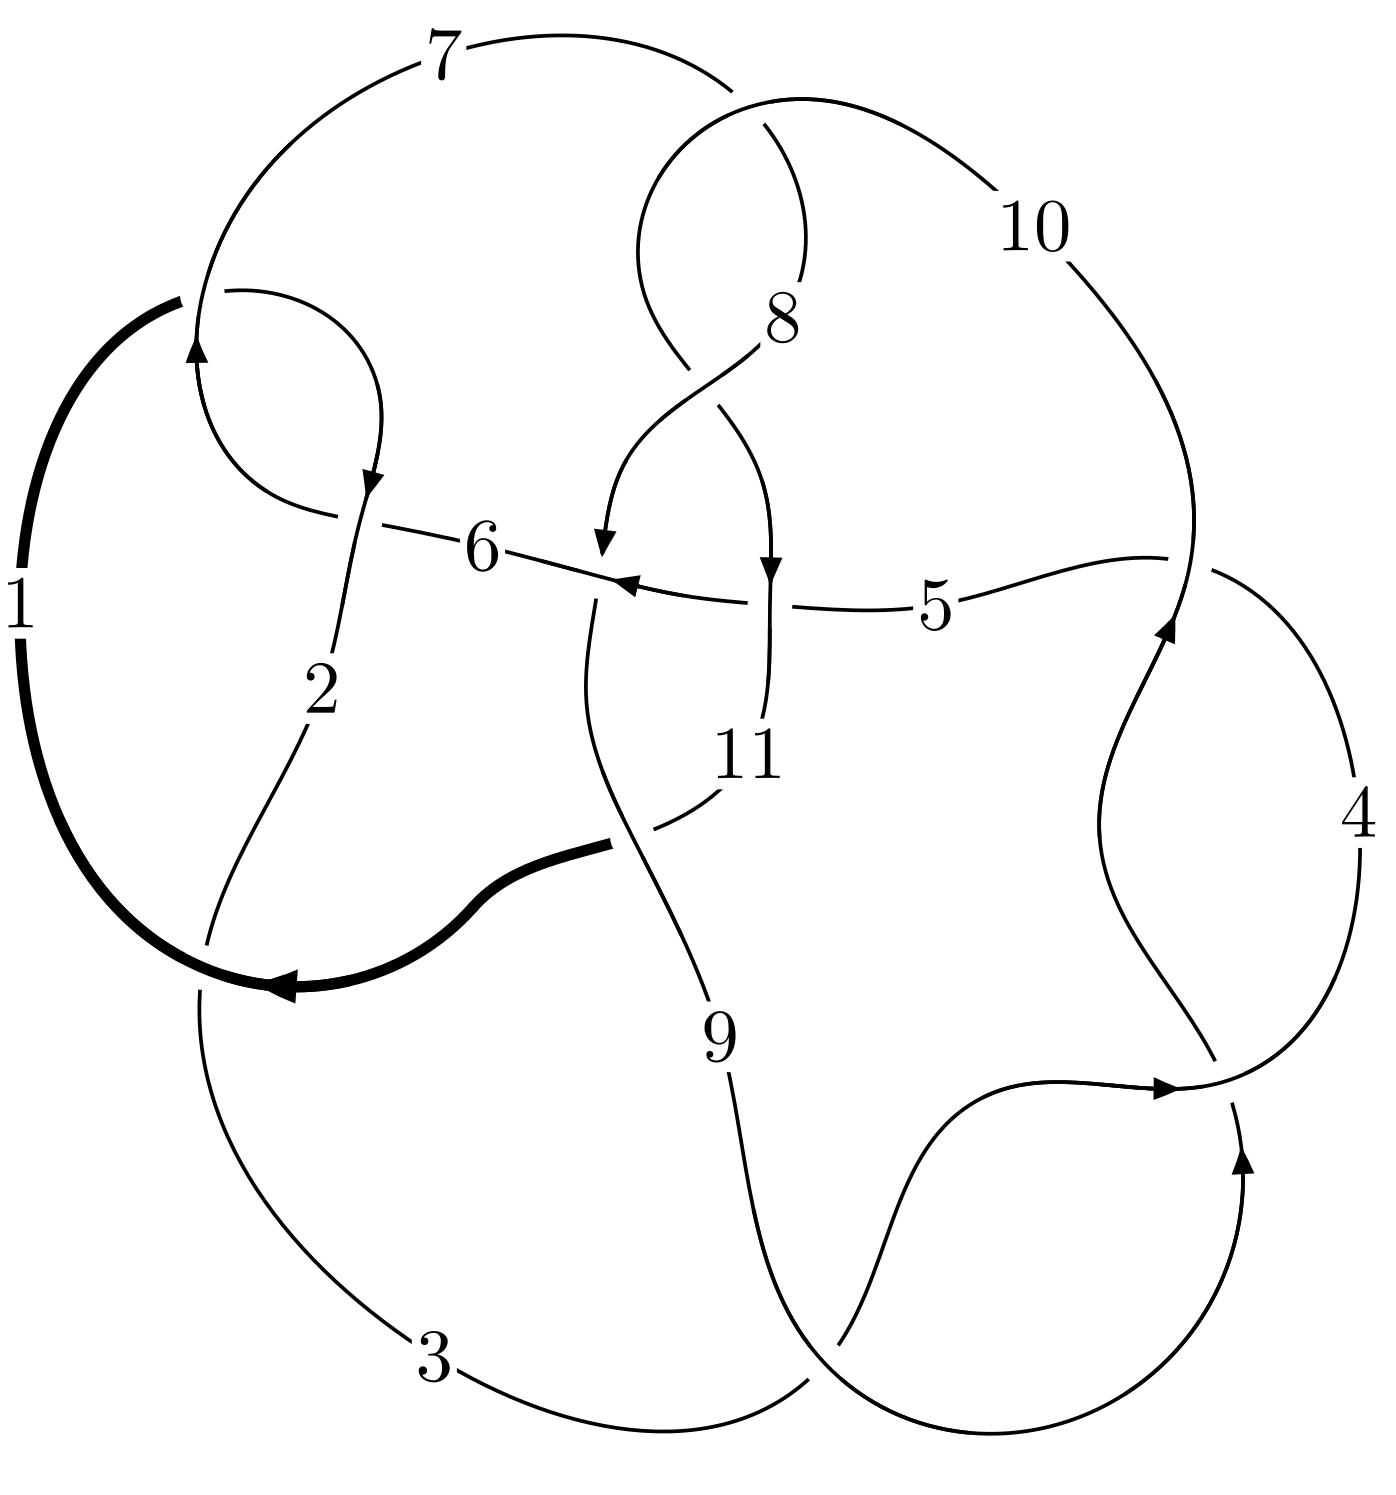
\includegraphics[width=112pt]{../../../GIT/diagram.site/Diagrams/png/741_11n_125.png}\\
\ \ \ A knot diagram\footnotemark}&
\allowdisplaybreaks
\textbf{Linearized knot diagam} \\
\cline{2-2}
 &
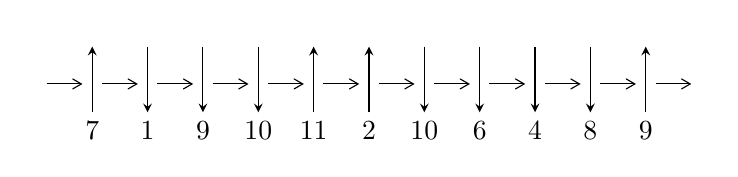
\begin{tikzpicture}[x=20pt, y=17pt]
	% nodes
	\node (C0) at (0, 0) {};
	\node (C1) at (1, 0) {};
	\node (C1U) at (1, +1) {};
	\node (C1D) at (1, -1) {7};

	\node (C2) at (2, 0) {};
	\node (C2U) at (2, +1) {};
	\node (C2D) at (2, -1) {1};

	\node (C3) at (3, 0) {};
	\node (C3U) at (3, +1) {};
	\node (C3D) at (3, -1) {9};

	\node (C4) at (4, 0) {};
	\node (C4U) at (4, +1) {};
	\node (C4D) at (4, -1) {10};

	\node (C5) at (5, 0) {};
	\node (C5U) at (5, +1) {};
	\node (C5D) at (5, -1) {11};

	\node (C6) at (6, 0) {};
	\node (C6U) at (6, +1) {};
	\node (C6D) at (6, -1) {2};

	\node (C7) at (7, 0) {};
	\node (C7U) at (7, +1) {};
	\node (C7D) at (7, -1) {10};

	\node (C8) at (8, 0) {};
	\node (C8U) at (8, +1) {};
	\node (C8D) at (8, -1) {6};

	\node (C9) at (9, 0) {};
	\node (C9U) at (9, +1) {};
	\node (C9D) at (9, -1) {4};

	\node (C10) at (10, 0) {};
	\node (C10U) at (10, +1) {};
	\node (C10D) at (10, -1) {8};

	\node (C11) at (11, 0) {};
	\node (C11U) at (11, +1) {};
	\node (C11D) at (11, -1) {9};
	\node (C12) at (12, 0) {};

	% arrows
	\draw[->,>={angle 60}]
	(C0) edge (C1) (C1) edge (C2) (C2) edge (C3) (C3) edge (C4) (C4) edge (C5) (C5) edge (C6) (C6) edge (C7) (C7) edge (C8) (C8) edge (C9) (C9) edge (C10) (C10) edge (C11) (C11) edge (C12) ;	\draw[->,>=stealth]
	(C1D) edge (C1U) (C2U) edge (C2D) (C3U) edge (C3D) (C4U) edge (C4D) (C5D) edge (C5U) (C6D) edge (C6U) (C7U) edge (C7D) (C8U) edge (C8D) (C9U) edge (C9D) (C10U) edge (C10D) (C11D) edge (C11U) ;
	\end{tikzpicture} \\
\hhline{~~} \\& 
\textbf{Solving Sequence} \\ \cline{2-2} 
 &
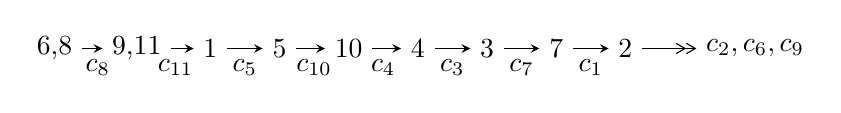
\begin{tikzpicture}[x=25pt, y=7pt]
	% node
	\node (A0) at (-1/8, 0) {6,8};
	\node (A1) at (17/16, 0) {9,11};
	\node (A2) at (17/8, 0) {1};
	\node (A3) at (25/8, 0) {5};
	\node (A4) at (33/8, 0) {10};
	\node (A5) at (41/8, 0) {4};
	\node (A6) at (49/8, 0) {3};
	\node (A7) at (57/8, 0) {7};
	\node (A8) at (65/8, 0) {2};
	\node (C1) at (1/2, -1) {$c_{8}$};
	\node (C2) at (13/8, -1) {$c_{11}$};
	\node (C3) at (21/8, -1) {$c_{5}$};
	\node (C4) at (29/8, -1) {$c_{10}$};
	\node (C5) at (37/8, -1) {$c_{4}$};
	\node (C6) at (45/8, -1) {$c_{3}$};
	\node (C7) at (53/8, -1) {$c_{7}$};
	\node (C8) at (61/8, -1) {$c_{1}$};
	\node (A9) at (10, 0) {$c_{2},c_{6},c_{9}$};

	% edge
	\draw[->,>=stealth]	
	(A0) edge (A1) (A1) edge (A2) (A2) edge (A3) (A3) edge (A4) (A4) edge (A5) (A5) edge (A6) (A6) edge (A7) (A7) edge (A8) ;
	\draw[->>,>={angle 60}]	
	(A8) edge (A9);
\end{tikzpicture} \\ 

\end{tabular} \\

\footnotetext{
The image of knot diagram is generated by the software ``\textbf{Draw programme}" developed by Andrew Bartholomew(\url{http://www.layer8.co.uk/maths/draw/index.htm\#Running-draw}), where we modified some parts for our purpose(\url{https://github.com/CATsTAILs/LinksPainter}).
}\phantom \\ \newline 
\centering \textbf{Ideals for irreducible components\footnotemark of $X_{\text{par}}$} 
 
\begin{align*}
I^u_{1}&=\langle 
3705 u^{16}-598 u^{15}+\cdots+73291 b-17911,\;6307 u^{16}+8497 u^{15}+\cdots+73291 a-25307,\\
\phantom{I^u_{1}}&\phantom{= \langle  }u^{17}- u^{16}+8 u^{13}-7 u^{12}+u^{11}+u^{10}+15 u^9-14 u^8- u^7+2 u^6+3 u^5+u^4-2 u^3-2 u^2+1\rangle \\
I^u_{2}&=\langle 
-1.62758\times10^{19} u^{23}-2.19259\times10^{19} u^{22}+\cdots+4.09578\times10^{18} b+4.17547\times10^{19},\\
\phantom{I^u_{2}}&\phantom{= \langle  }1.02456\times10^{19} u^{23}+1.20636\times10^{19} u^{22}+\cdots+1.10459\times10^{18} a-5.53806\times10^{19},\;u^{24}+u^{23}+\cdots-12 u+1\rangle \\
I^u_{3}&=\langle 
- u^8- u^7+3 u^6+3 u^5- u^4-2 u^3-2 u^2+b,\;u^8+u^7-4 u^6-4 u^5+4 u^4+5 u^3+u^2+a-2 u-1,\\
\phantom{I^u_{3}}&\phantom{= \langle  }u^{10}+u^9-4 u^8-4 u^7+4 u^6+5 u^5+u^4-2 u^3-2 u^2+1\rangle \\
\\
\end{align*}
\raggedright * 3 irreducible components of $\dim_{\mathbb{C}}=0$, with total 51 representations.\\
\footnotetext{All coefficients of polynomials are rational numbers. But the coefficients are sometimes approximated in decimal forms when there is not enough margin.}
\newpage
\renewcommand{\arraystretch}{1}
\centering \section*{I. $I^u_{1}= \langle 3705 u^{16}-598 u^{15}+\cdots+73291 b-17911,\;6307 u^{16}+8497 u^{15}+\cdots+73291 a-25307,\;u^{17}- u^{16}+\cdots-2 u^2+1 \rangle$}
\flushleft \textbf{(i) Arc colorings}\\
\begin{tabular}{m{7pt} m{180pt} m{7pt} m{180pt} }
\flushright $a_{6}=$&$\begin{pmatrix}0\\u\end{pmatrix}$ \\
\flushright $a_{8}=$&$\begin{pmatrix}1\\0\end{pmatrix}$ \\
\flushright $a_{9}=$&$\begin{pmatrix}1\\u^2\end{pmatrix}$ \\
\flushright $a_{11}=$&$\begin{pmatrix}-0.0860542 u^{16}-0.115935 u^{15}+\cdots-0.529669 u+0.345295\\-0.0505519 u^{16}+0.00815926 u^{15}+\cdots+0.136606 u+0.244382\end{pmatrix}$ \\
\flushright $a_{1}=$&$\begin{pmatrix}-0.0233589 u^{16}-0.00324733 u^{15}+\cdots-0.479117 u+0.387687\\0.198278 u^{16}-0.0425291 u^{15}+\cdots+0.0739108 u+0.0689989\end{pmatrix}$ \\
\flushright $a_{5}=$&$\begin{pmatrix}0.654705 u^{16}-0.740759 u^{15}+\cdots-0.188099 u-0.529669\\-0.201989 u^{16}+0.0887421 u^{15}+\cdots+0.345295 u+0.0860542\end{pmatrix}$ \\
\flushright $a_{10}=$&$\begin{pmatrix}-0.136606 u^{16}-0.107776 u^{15}+\cdots-0.393063 u+0.589677\\-0.0505519 u^{16}+0.00815926 u^{15}+\cdots+0.136606 u+0.244382\end{pmatrix}$ \\
\flushright $a_{4}=$&$\begin{pmatrix}0.410323 u^{16}-0.546929 u^{15}+\cdots+0.401577 u-0.393063\\-0.244382 u^{16}+0.193830 u^{15}+\cdots+0.589677 u+0.136606\end{pmatrix}$ \\
\flushright $a_{3}=$&$\begin{pmatrix}0.410323 u^{16}-0.546929 u^{15}+\cdots+1.40158 u-0.393063\\-0.244382 u^{16}+0.193830 u^{15}+\cdots+0.589677 u+0.136606\end{pmatrix}$ \\
\flushright $a_{7}=$&$\begin{pmatrix}-0.968809 u^{16}+0.0160183 u^{15}+\cdots+0.388588 u+1.25569\\-0.882755 u^{16}+0.131953 u^{15}+\cdots+0.918257 u+0.910398\end{pmatrix}$ \\
\flushright $a_{2}=$&$\begin{pmatrix}1.43914 u^{16}-0.141054 u^{15}+\cdots-4.14755 u-2.06759\\2.34525 u^{16}-0.269760 u^{15}+\cdots-4.58669 u-3.36568\end{pmatrix}$\\ \flushright $a_{2}=$&$\begin{pmatrix}1.43914 u^{16}-0.141054 u^{15}+\cdots-4.14755 u-2.06759\\2.34525 u^{16}-0.269760 u^{15}+\cdots-4.58669 u-3.36568\end{pmatrix}$\\&\end{tabular}
\flushleft \textbf{(ii) Obstruction class $= -1$}\\~\\
\flushleft \textbf{(iii) Cusp Shapes $= \frac{112951}{73291} u^{16}+\frac{78462}{73291} u^{15}+\cdots-\frac{754923}{73291} u-\frac{768857}{73291}$}\\~\\
\newpage\renewcommand{\arraystretch}{1}
\flushleft \textbf{(iv) u-Polynomials at the component}\newline \\
\begin{tabular}{m{50pt}|m{274pt}}
Crossings & \hspace{64pt}u-Polynomials at each crossing \\
\hline $$\begin{aligned}c_{1},c_{6}\end{aligned}$$&$\begin{aligned}
&u^{17}+6 u^{16}+\cdots+32 u+8
\end{aligned}$\\
\hline $$\begin{aligned}c_{2}\end{aligned}$$&$\begin{aligned}
&u^{17}+6 u^{16}+\cdots+32 u-64
\end{aligned}$\\
\hline $$\begin{aligned}c_{3},c_{4},c_{8}\\c_{9}\end{aligned}$$&$\begin{aligned}
&u^{17}- u^{16}+\cdots-2 u^2+1
\end{aligned}$\\
\hline $$\begin{aligned}c_{5}\end{aligned}$$&$\begin{aligned}
&u^{17}+u^{16}+\cdots-22 u^2+1
\end{aligned}$\\
\hline $$\begin{aligned}c_{7},c_{10}\end{aligned}$$&$\begin{aligned}
&u^{17}-7 u^{16}+\cdots-80 u+16
\end{aligned}$\\
\hline $$\begin{aligned}c_{11}\end{aligned}$$&$\begin{aligned}
&u^{17}+3 u^{16}+\cdots+4 u+1
\end{aligned}$\\
\hline
\end{tabular}\\~\\
\newpage\renewcommand{\arraystretch}{1}
\flushleft \textbf{(v) Riley Polynomials at the component}\newline \\
\begin{tabular}{m{50pt}|m{274pt}}
Crossings & \hspace{64pt}Riley Polynomials at each crossing \\
\hline $$\begin{aligned}c_{1},c_{6}\end{aligned}$$&$\begin{aligned}
&y^{17}+6 y^{16}+\cdots+32 y-64
\end{aligned}$\\
\hline $$\begin{aligned}c_{2}\end{aligned}$$&$\begin{aligned}
&y^{17}+10 y^{16}+\cdots+33280 y-4096
\end{aligned}$\\
\hline $$\begin{aligned}c_{3},c_{4},c_{8}\\c_{9}\end{aligned}$$&$\begin{aligned}
&y^{17}- y^{16}+\cdots+4 y-1
\end{aligned}$\\
\hline $$\begin{aligned}c_{5}\end{aligned}$$&$\begin{aligned}
&y^{17}-13 y^{16}+\cdots+44 y-1
\end{aligned}$\\
\hline $$\begin{aligned}c_{7},c_{10}\end{aligned}$$&$\begin{aligned}
&y^{17}-7 y^{16}+\cdots-128 y-256
\end{aligned}$\\
\hline $$\begin{aligned}c_{11}\end{aligned}$$&$\begin{aligned}
&y^{17}-27 y^{16}+\cdots-24 y-1
\end{aligned}$\\
\hline
\end{tabular}\\~\\
\newpage\flushleft \textbf{(vi) Complex Volumes and Cusp Shapes}
$$\begin{array}{c|c|c}  
\text{Solutions to }I^u_{1}& \I (\text{vol} + \sqrt{-1}CS) & \text{Cusp shape}\\
 \hline 
\begin{aligned}
u &= \phantom{-}0.724405 + 0.548318 I \\
a &= -0.75306 + 1.73640 I \\
b &= -1.210220 - 0.484731 I\end{aligned}
 & -4.29085 - 6.01779 I & -7.18678 + 9.97359 I \\ \hline\begin{aligned}
u &= \phantom{-}0.724405 - 0.548318 I \\
a &= -0.75306 - 1.73640 I \\
b &= -1.210220 + 0.484731 I\end{aligned}
 & -4.29085 + 6.01779 I & -7.18678 - 9.97359 I \\ \hline\begin{aligned}
u &= -0.126925 + 0.721173 I \\
a &= \phantom{-}0.84923 - 1.76296 I \\
b &= -0.778224 + 0.460398 I\end{aligned}
 & \phantom{-}1.34232 + 1.94872 I & \phantom{-}2.56083 - 3.14210 I \\ \hline\begin{aligned}
u &= -0.126925 - 0.721173 I \\
a &= \phantom{-}0.84923 + 1.76296 I \\
b &= -0.778224 - 0.460398 I\end{aligned}
 & \phantom{-}1.34232 - 1.94872 I & \phantom{-}2.56083 + 3.14210 I \\ \hline\begin{aligned}
u &= \phantom{-}0.725128 + 0.055021 I \\
a &= \phantom{-}0.394130 - 0.065047 I \\
b &= \phantom{-}1.46996 + 0.40764 I\end{aligned}
 & -4.56765 - 3.93288 I & -12.22005 + 0.69203 I \\ \hline\begin{aligned}
u &= \phantom{-}0.725128 - 0.055021 I \\
a &= \phantom{-}0.394130 + 0.065047 I \\
b &= \phantom{-}1.46996 - 0.40764 I\end{aligned}
 & -4.56765 + 3.93288 I & -12.22005 - 0.69203 I \\ \hline\begin{aligned}
u &= \phantom{-}0.746984 + 1.046150 I \\
a &= \phantom{-}0.322934 - 0.862372 I \\
b &= -0.619169 + 1.016980 I\end{aligned}
 & \phantom{-}6.33629 - 0.97017 I & -0.559057 + 0.284542 I \\ \hline\begin{aligned}
u &= \phantom{-}0.746984 - 1.046150 I \\
a &= \phantom{-}0.322934 + 0.862372 I \\
b &= -0.619169 - 1.016980 I\end{aligned}
 & \phantom{-}6.33629 + 0.97017 I & -0.559057 - 0.284542 I \\ \hline\begin{aligned}
u &= -0.909916 + 0.943922 I \\
a &= \phantom{-}0.275853 + 0.793772 I \\
b &= -0.609367 - 1.124050 I\end{aligned}
 & \phantom{-}5.27663 + 7.20759 I & -2.52796 - 5.51575 I \\ \hline\begin{aligned}
u &= -0.909916 - 0.943922 I \\
a &= \phantom{-}0.275853 - 0.793772 I \\
b &= -0.609367 + 1.124050 I\end{aligned}
 & \phantom{-}5.27663 - 7.20759 I & -2.52796 + 5.51575 I\\
 \hline 
 \end{array}$$\newpage$$\begin{array}{c|c|c}  
\text{Solutions to }I^u_{1}& \I (\text{vol} + \sqrt{-1}CS) & \text{Cusp shape}\\
 \hline 
\begin{aligned}
u &= -0.512854 + 0.417660 I \\
a &= \phantom{-}0.640794 + 0.460951 I \\
b &= \phantom{-}0.028408 - 0.739779 I\end{aligned}
 & -0.81159 + 1.48098 I & -4.11600 - 4.97481 I \\ \hline\begin{aligned}
u &= -0.512854 - 0.417660 I \\
a &= \phantom{-}0.640794 - 0.460951 I \\
b &= \phantom{-}0.028408 + 0.739779 I\end{aligned}
 & -0.81159 - 1.48098 I & -4.11600 + 4.97481 I \\ \hline\begin{aligned}
u &= -0.641391\phantom{ +0.000000I} \\
a &= \phantom{-}0.489889\phantom{ +0.000000I} \\
b &= \phantom{-}1.04128\phantom{ +0.000000I}\end{aligned}
 & -1.52652\phantom{ +0.000000I} & -7.18720\phantom{ +0.000000I} \\ \hline\begin{aligned}
u &= -1.05004 + 1.03914 I \\
a &= -0.221763 - 1.275910 I \\
b &= -1.132230 + 0.760774 I\end{aligned}
 & \phantom{-}4.69624 + 7.43319 I & -2.80359 - 4.35460 I \\ \hline\begin{aligned}
u &= -1.05004 - 1.03914 I \\
a &= -0.221763 + 1.275910 I \\
b &= -1.132230 - 0.760774 I\end{aligned}
 & \phantom{-}4.69624 - 7.43319 I & -2.80359 + 4.35460 I \\ \hline\begin{aligned}
u &= \phantom{-}1.22392 + 0.97901 I \\
a &= -0.253054 + 1.194280 I \\
b &= -1.16979 - 0.80134 I\end{aligned}
 & \phantom{-}3.4739 - 14.0835 I & -4.55379 + 8.21992 I \\ \hline\begin{aligned}
u &= \phantom{-}1.22392 - 0.97901 I \\
a &= -0.253054 - 1.194280 I \\
b &= -1.16979 + 0.80134 I\end{aligned}
 & \phantom{-}3.4739 + 14.0835 I & -4.55379 - 8.21992 I\\
 \hline 
 \end{array}$$\newpage\newpage\renewcommand{\arraystretch}{1}
\centering \section*{II. $I^u_{2}= \langle -1.63\times10^{19} u^{23}-2.19\times10^{19} u^{22}+\cdots+4.10\times10^{18} b+4.18\times10^{19},\;1.02\times10^{19} u^{23}+1.21\times10^{19} u^{22}+\cdots+1.10\times10^{18} a-5.54\times10^{19},\;u^{24}+u^{23}+\cdots-12 u+1 \rangle$}
\flushleft \textbf{(i) Arc colorings}\\
\begin{tabular}{m{7pt} m{180pt} m{7pt} m{180pt} }
\flushright $a_{6}=$&$\begin{pmatrix}0\\u\end{pmatrix}$ \\
\flushright $a_{8}=$&$\begin{pmatrix}1\\0\end{pmatrix}$ \\
\flushright $a_{9}=$&$\begin{pmatrix}1\\u^2\end{pmatrix}$ \\
\flushright $a_{11}=$&$\begin{pmatrix}-9.27552 u^{23}-10.9214 u^{22}+\cdots-365.606 u+50.1368\\3.97380 u^{23}+5.35329 u^{22}+\cdots+100.403 u-10.1946\end{pmatrix}$ \\
\flushright $a_{1}=$&$\begin{pmatrix}-4.82541 u^{23}-4.75510 u^{22}+\cdots-254.728 u+38.2964\\4.74826 u^{23}+6.65968 u^{22}+\cdots+116.547 u-11.9107\end{pmatrix}$ \\
\flushright $a_{5}=$&$\begin{pmatrix}11.3054 u^{23}+12.3377 u^{22}+\cdots+440.071 u-45.2263\\6.36090 u^{23}+7.80155 u^{22}+\cdots+204.414 u-23.9970\end{pmatrix}$ \\
\flushright $a_{10}=$&$\begin{pmatrix}-5.30172 u^{23}-5.56808 u^{22}+\cdots-265.203 u+39.9422\\3.97380 u^{23}+5.35329 u^{22}+\cdots+100.403 u-10.1946\end{pmatrix}$ \\
\flushright $a_{4}=$&$\begin{pmatrix}14.7955 u^{23}+17.5151 u^{22}+\cdots+528.748 u-61.5891\\-0.682634 u^{23}-1.19757 u^{22}+\cdots-4.09647 u-0.631997\end{pmatrix}$ \\
\flushright $a_{3}=$&$\begin{pmatrix}13.8574 u^{23}+16.1229 u^{22}+\cdots+506.811 u-59.5014\\-0.936526 u^{23}-1.63331 u^{22}+\cdots-8.60722 u-0.177923\end{pmatrix}$ \\
\flushright $a_{7}=$&$\begin{pmatrix}17.3035 u^{23}+22.0294 u^{22}+\cdots+507.574 u-57.5598\\-6.69344 u^{23}-8.32845 u^{22}+\cdots-216.360 u+25.9901\end{pmatrix}$ \\
\flushright $a_{2}=$&$\begin{pmatrix}-7.27158 u^{23}-9.66160 u^{22}+\cdots-203.491 u+24.3547\\2.43276 u^{23}+3.92231 u^{22}+\cdots+34.3850 u-0.488514\end{pmatrix}$\\ \flushright $a_{2}=$&$\begin{pmatrix}-7.27158 u^{23}-9.66160 u^{22}+\cdots-203.491 u+24.3547\\2.43276 u^{23}+3.92231 u^{22}+\cdots+34.3850 u-0.488514\end{pmatrix}$\\&\end{tabular}
\flushleft \textbf{(ii) Obstruction class $= -1$}\\~\\
\flushleft \textbf{(iii) Cusp Shapes $= -\frac{5816969908025562256904}{462822645525235397669} u^{23}-\frac{6619395108009854597496}{462822645525235397669} u^{22}+\cdots-\frac{12260288530768323150784}{27224861501484435157} u+\frac{21994338350330534399466}{462822645525235397669}$}\\~\\
\newpage\renewcommand{\arraystretch}{1}
\flushleft \textbf{(iv) u-Polynomials at the component}\newline \\
\begin{tabular}{m{50pt}|m{274pt}}
Crossings & \hspace{64pt}u-Polynomials at each crossing \\
\hline $$\begin{aligned}c_{1},c_{6}\end{aligned}$$&$\begin{aligned}
&(u^4- u^3+u^2+1)^6
\end{aligned}$\\
\hline $$\begin{aligned}c_{2}\end{aligned}$$&$\begin{aligned}
&(u^4+u^3+3 u^2+2 u+1)^6
\end{aligned}$\\
\hline $$\begin{aligned}c_{3},c_{4},c_{8}\\c_{9}\end{aligned}$$&$\begin{aligned}
&u^{24}+u^{23}+\cdots-12 u+1
\end{aligned}$\\
\hline $$\begin{aligned}c_{5}\end{aligned}$$&$\begin{aligned}
&u^{24}+3 u^{23}+\cdots+54 u+107
\end{aligned}$\\
\hline $$\begin{aligned}c_{7},c_{10}\end{aligned}$$&$\begin{aligned}
&(u^3+u^2-1)^8
\end{aligned}$\\
\hline $$\begin{aligned}c_{11}\end{aligned}$$&$\begin{aligned}
&u^{24}+3 u^{23}+\cdots+846 u+347
\end{aligned}$\\
\hline
\end{tabular}\\~\\
\newpage\renewcommand{\arraystretch}{1}
\flushleft \textbf{(v) Riley Polynomials at the component}\newline \\
\begin{tabular}{m{50pt}|m{274pt}}
Crossings & \hspace{64pt}Riley Polynomials at each crossing \\
\hline $$\begin{aligned}c_{1},c_{6}\end{aligned}$$&$\begin{aligned}
&(y^4+y^3+3 y^2+2 y+1)^6
\end{aligned}$\\
\hline $$\begin{aligned}c_{2}\end{aligned}$$&$\begin{aligned}
&(y^4+5 y^3+7 y^2+2 y+1)^6
\end{aligned}$\\
\hline $$\begin{aligned}c_{3},c_{4},c_{8}\\c_{9}\end{aligned}$$&$\begin{aligned}
&y^{24}-9 y^{23}+\cdots-40 y+1
\end{aligned}$\\
\hline $$\begin{aligned}c_{5}\end{aligned}$$&$\begin{aligned}
&y^{24}+3 y^{23}+\cdots+23192 y+11449
\end{aligned}$\\
\hline $$\begin{aligned}c_{7},c_{10}\end{aligned}$$&$\begin{aligned}
&(y^3- y^2+2 y-1)^8
\end{aligned}$\\
\hline $$\begin{aligned}c_{11}\end{aligned}$$&$\begin{aligned}
&y^{24}-9 y^{23}+\cdots+602884 y+120409
\end{aligned}$\\
\hline
\end{tabular}\\~\\
\newpage\flushleft \textbf{(vi) Complex Volumes and Cusp Shapes}
$$\begin{array}{c|c|c}  
\text{Solutions to }I^u_{2}& \I (\text{vol} + \sqrt{-1}CS) & \text{Cusp shape}\\
 \hline 
\begin{aligned}
u &= \phantom{-}1.008370 + 0.230741 I \\
a &= \phantom{-}0.324592 - 1.318030 I \\
b &= \phantom{-}0.877439 + 0.744862 I\end{aligned}
 & -2.12168 - 4.24323 I & -6.31698 + 7.88819 I \\ \hline\begin{aligned}
u &= \phantom{-}1.008370 - 0.230741 I \\
a &= \phantom{-}0.324592 + 1.318030 I \\
b &= \phantom{-}0.877439 - 0.744862 I\end{aligned}
 & -2.12168 + 4.24323 I & -6.31698 - 7.88819 I \\ \hline\begin{aligned}
u &= -0.430835 + 0.856235 I \\
a &= -0.577262 + 0.850887 I \\
b &= \phantom{-}0.877439 - 0.744862 I\end{aligned}
 & -2.12168 + 4.24323 I & -6.31698 - 7.88819 I \\ \hline\begin{aligned}
u &= -0.430835 - 0.856235 I \\
a &= -0.577262 - 0.850887 I \\
b &= \phantom{-}0.877439 + 0.744862 I\end{aligned}
 & -2.12168 - 4.24323 I & -6.31698 + 7.88819 I \\ \hline\begin{aligned}
u &= -0.324811 + 1.039220 I \\
a &= \phantom{-}1.271110 - 0.441707 I \\
b &= -0.754878\phantom{ +0.000000I}\end{aligned}
 & \phantom{-}0.74248 + 3.16396 I & -9.19277 - 2.56480 I \\ \hline\begin{aligned}
u &= -0.324811 - 1.039220 I \\
a &= \phantom{-}1.271110 + 0.441707 I \\
b &= -0.754878\phantom{ +0.000000I}\end{aligned}
 & \phantom{-}0.74248 - 3.16396 I & -9.19277 + 2.56480 I \\ \hline\begin{aligned}
u &= -1.003940 + 0.452899 I \\
a &= \phantom{-}0.012479 + 0.854104 I \\
b &= \phantom{-}0.877439 - 0.744862 I\end{aligned}
 & -2.12168 + 1.41302 I & -6.31698 + 1.92930 I \\ \hline\begin{aligned}
u &= -1.003940 - 0.452899 I \\
a &= \phantom{-}0.012479 - 0.854104 I \\
b &= \phantom{-}0.877439 + 0.744862 I\end{aligned}
 & -2.12168 - 1.41302 I & -6.31698 - 1.92930 I \\ \hline\begin{aligned}
u &= \phantom{-}1.382990 + 0.000366 I \\
a &= -0.948443 - 0.485387 I \\
b &= -0.754878\phantom{ +0.000000I}\end{aligned}
 & -6.25926 - 1.41510 I & -12.84625 + 4.90874 I \\ \hline\begin{aligned}
u &= \phantom{-}1.382990 - 0.000366 I \\
a &= -0.948443 + 0.485387 I \\
b &= -0.754878\phantom{ +0.000000I}\end{aligned}
 & -6.25926 + 1.41510 I & -12.84625 - 4.90874 I\\
 \hline 
 \end{array}$$\newpage$$\begin{array}{c|c|c}  
\text{Solutions to }I^u_{2}& \I (\text{vol} + \sqrt{-1}CS) & \text{Cusp shape}\\
 \hline 
\begin{aligned}
u &= -1.043140 + 0.911052 I \\
a &= \phantom{-}0.738284 + 1.097470 I \\
b &= \phantom{-}0.877439 - 0.744862 I\end{aligned}
 & \phantom{-}4.88007 - 0.33584 I & -2.66351 - 0.41465 I \\ \hline\begin{aligned}
u &= -1.043140 - 0.911052 I \\
a &= \phantom{-}0.738284 - 1.097470 I \\
b &= \phantom{-}0.877439 + 0.744862 I\end{aligned}
 & \phantom{-}4.88007 + 0.33584 I & -2.66351 + 0.41465 I \\ \hline\begin{aligned}
u &= \phantom{-}1.19721 + 0.83587 I \\
a &= \phantom{-}0.694157 - 1.132290 I \\
b &= \phantom{-}0.877439 + 0.744862 I\end{aligned}
 & \phantom{-}4.88007 - 5.99209 I & -2.66351 + 5.54425 I \\ \hline\begin{aligned}
u &= \phantom{-}1.19721 - 0.83587 I \\
a &= \phantom{-}0.694157 + 1.132290 I \\
b &= \phantom{-}0.877439 - 0.744862 I\end{aligned}
 & \phantom{-}4.88007 + 5.99209 I & -2.66351 - 5.54425 I \\ \hline\begin{aligned}
u &= -1.00875 + 1.10787 I \\
a &= -0.390615 - 0.422077 I \\
b &= \phantom{-}0.877439 + 0.744862 I\end{aligned}
 & \phantom{-}4.88007 + 0.33584 I & -2.66351 + 0.41465 I \\ \hline\begin{aligned}
u &= -1.00875 - 1.10787 I \\
a &= -0.390615 + 0.422077 I \\
b &= \phantom{-}0.877439 - 0.744862 I\end{aligned}
 & \phantom{-}4.88007 - 0.33584 I & -2.66351 - 0.41465 I \\ \hline\begin{aligned}
u &= \phantom{-}0.80956 + 1.30687 I \\
a &= -0.428288 + 0.453956 I \\
b &= \phantom{-}0.877439 - 0.744862 I\end{aligned}
 & \phantom{-}4.88007 + 5.99209 I & -2.66351 - 5.54425 I \\ \hline\begin{aligned}
u &= \phantom{-}0.80956 - 1.30687 I \\
a &= -0.428288 - 0.453956 I \\
b &= \phantom{-}0.877439 + 0.744862 I\end{aligned}
 & \phantom{-}4.88007 - 5.99209 I & -2.66351 + 5.54425 I \\ \hline\begin{aligned}
u &= -1.60815 + 0.28919 I \\
a &= -0.181824 - 0.347739 I \\
b &= -0.754878\phantom{ +0.000000I}\end{aligned}
 & -6.25926 + 1.41510 I & -12.84625 - 4.90874 I \\ \hline\begin{aligned}
u &= -1.60815 - 0.28919 I \\
a &= -0.181824 + 0.347739 I \\
b &= -0.754878\phantom{ +0.000000I}\end{aligned}
 & -6.25926 - 1.41510 I & -12.84625 + 4.90874 I\\
 \hline 
 \end{array}$$\newpage$$\begin{array}{c|c|c}  
\text{Solutions to }I^u_{2}& \I (\text{vol} + \sqrt{-1}CS) & \text{Cusp shape}\\
 \hline 
\begin{aligned}
u &= \phantom{-}0.265048 + 0.154544 I \\
a &= -4.33744 - 5.56259 I \\
b &= -0.754878\phantom{ +0.000000I}\end{aligned}
 & \phantom{-}0.74248 - 3.16396 I & -9.19277 + 2.56480 I \\ \hline\begin{aligned}
u &= \phantom{-}0.265048 - 0.154544 I \\
a &= -4.33744 + 5.56259 I \\
b &= -0.754878\phantom{ +0.000000I}\end{aligned}
 & \phantom{-}0.74248 + 3.16396 I & -9.19277 - 2.56480 I \\ \hline\begin{aligned}
u &= \phantom{-}0.256438 + 0.045429 I \\
a &= -0.67675 - 3.40086 I \\
b &= \phantom{-}0.877439 + 0.744862 I\end{aligned}
 & -2.12168 - 1.41302 I & -6.31698 - 1.92930 I \\ \hline\begin{aligned}
u &= \phantom{-}0.256438 - 0.045429 I \\
a &= -0.67675 + 3.40086 I \\
b &= \phantom{-}0.877439 - 0.744862 I\end{aligned}
 & -2.12168 + 1.41302 I & -6.31698 + 1.92930 I\\
 \hline 
 \end{array}$$\newpage\newpage\renewcommand{\arraystretch}{1}
\centering \section*{III. $I^u_{3}= \langle - u^8- u^7+3 u^6+3 u^5- u^4-2 u^3-2 u^2+b,\;u^8+u^7+\cdots+a-1,\;u^{10}+u^9+\cdots-2 u^2+1 \rangle$}
\flushleft \textbf{(i) Arc colorings}\\
\begin{tabular}{m{7pt} m{180pt} m{7pt} m{180pt} }
\flushright $a_{6}=$&$\begin{pmatrix}0\\u\end{pmatrix}$ \\
\flushright $a_{8}=$&$\begin{pmatrix}1\\0\end{pmatrix}$ \\
\flushright $a_{9}=$&$\begin{pmatrix}1\\u^2\end{pmatrix}$ \\
\flushright $a_{11}=$&$\begin{pmatrix}- u^8- u^7+4 u^6+4 u^5-4 u^4-5 u^3- u^2+2 u+1\\u^8+u^7-3 u^6-3 u^5+u^4+2 u^3+2 u^2\end{pmatrix}$ \\
\flushright $a_{1}=$&$\begin{pmatrix}u^6+u^5-3 u^4-3 u^3+2 u^2+2 u\\2 u^8+2 u^7-6 u^6-6 u^5+3 u^4+4 u^3+3 u^2-1\end{pmatrix}$ \\
\flushright $a_{5}=$&$\begin{pmatrix}u^7+u^6-4 u^5-4 u^4+4 u^3+5 u^2-2\\u^9+u^8-4 u^7-4 u^6+4 u^5+5 u^4+u^3-2 u^2- u\end{pmatrix}$ \\
\flushright $a_{10}=$&$\begin{pmatrix}u^6+u^5-3 u^4-3 u^3+u^2+2 u+1\\u^8+u^7-3 u^6-3 u^5+u^4+2 u^3+2 u^2\end{pmatrix}$ \\
\flushright $a_{4}=$&$\begin{pmatrix}- u^5- u^4+3 u^3+3 u^2- u-2\\- u^7- u^6+3 u^5+3 u^4- u^3-2 u^2- u\end{pmatrix}$ \\
\flushright $a_{3}=$&$\begin{pmatrix}- u^5- u^4+3 u^3+3 u^2-2 u-2\\- u^7- u^6+3 u^5+3 u^4-2 u^3-2 u^2- u\end{pmatrix}$ \\
\flushright $a_{7}=$&$\begin{pmatrix}u^4+u^3-2 u^2-2 u\\- u^8- u^7+4 u^6+4 u^5-3 u^4-4 u^3-3 u^2+1\end{pmatrix}$ \\
\flushright $a_{2}=$&$\begin{pmatrix}u^9+2 u^8-3 u^7-7 u^6+u^5+6 u^4+3 u^3+u^2- u-1\\u^9+3 u^8-2 u^7-10 u^6-2 u^5+8 u^4+6 u^3+2 u^2-3 u-2\end{pmatrix}$\\ \flushright $a_{2}=$&$\begin{pmatrix}u^9+2 u^8-3 u^7-7 u^6+u^5+6 u^4+3 u^3+u^2- u-1\\u^9+3 u^8-2 u^7-10 u^6-2 u^5+8 u^4+6 u^3+2 u^2-3 u-2\end{pmatrix}$\\&\end{tabular}
\flushleft \textbf{(ii) Obstruction class $= 1$}\\~\\
\flushleft \textbf{(iii) Cusp Shapes $= - u^9+4 u^8+10 u^7-18 u^6-30 u^5+17 u^4+30 u^3+10 u^2-8 u-15$}\\~\\
\newpage\renewcommand{\arraystretch}{1}
\flushleft \textbf{(iv) u-Polynomials at the component}\newline \\
\begin{tabular}{m{50pt}|m{274pt}}
Crossings & \hspace{64pt}u-Polynomials at each crossing \\
\hline $$\begin{aligned}c_{1}\end{aligned}$$&$\begin{aligned}
&u^{10}+u^9+3 u^8+2 u^7+5 u^6+2 u^5+5 u^4+3 u^2+1
\end{aligned}$\\
\hline $$\begin{aligned}c_{2}\end{aligned}$$&$\begin{aligned}
&u^{10}+5 u^9+\cdots+6 u+1
\end{aligned}$\\
\hline $$\begin{aligned}c_{3},c_{4},c_{8}\end{aligned}$$&$\begin{aligned}
&u^{10}+u^9-4 u^8-4 u^7+4 u^6+5 u^5+u^4-2 u^3-2 u^2+1
\end{aligned}$\\
\hline $$\begin{aligned}c_{5}\end{aligned}$$&$\begin{aligned}
&u^{10}+u^9+4 u^8+5 u^7+2 u^6- u^3-2 u^2+1
\end{aligned}$\\
\hline $$\begin{aligned}c_{6}\end{aligned}$$&$\begin{aligned}
&u^{10}- u^9+3 u^8-2 u^7+5 u^6-2 u^5+5 u^4+3 u^2+1
\end{aligned}$\\
\hline $$\begin{aligned}c_{7}\end{aligned}$$&$\begin{aligned}
&u^{10}-2 u^9- u^8+6 u^7-2 u^6-7 u^5+6 u^4+4 u^3-4 u^2- u+1
\end{aligned}$\\
\hline $$\begin{aligned}c_{9}\end{aligned}$$&$\begin{aligned}
&u^{10}- u^9-4 u^8+4 u^7+4 u^6-5 u^5+u^4+2 u^3-2 u^2+1
\end{aligned}$\\
\hline $$\begin{aligned}c_{10}\end{aligned}$$&$\begin{aligned}
&u^{10}+2 u^9- u^8-6 u^7-2 u^6+7 u^5+6 u^4-4 u^3-4 u^2+u+1
\end{aligned}$\\
\hline $$\begin{aligned}c_{11}\end{aligned}$$&$\begin{aligned}
&u^{10}+u^9+3 u^8+u^6-2 u^5+3 u^4+u^3+2 u^2+1
\end{aligned}$\\
\hline
\end{tabular}\\~\\
\newpage\renewcommand{\arraystretch}{1}
\flushleft \textbf{(v) Riley Polynomials at the component}\newline \\
\begin{tabular}{m{50pt}|m{274pt}}
Crossings & \hspace{64pt}Riley Polynomials at each crossing \\
\hline $$\begin{aligned}c_{1},c_{6}\end{aligned}$$&$\begin{aligned}
&y^{10}+5 y^9+\cdots+6 y+1
\end{aligned}$\\
\hline $$\begin{aligned}c_{2}\end{aligned}$$&$\begin{aligned}
&y^{10}+5 y^9+\cdots+2 y+1
\end{aligned}$\\
\hline $$\begin{aligned}c_{3},c_{4},c_{8}\\c_{9}\end{aligned}$$&$\begin{aligned}
&y^{10}-9 y^9+32 y^8-56 y^7+48 y^6-15 y^5-3 y^4+6 y^2-4 y+1
\end{aligned}$\\
\hline $$\begin{aligned}c_{5}\end{aligned}$$&$\begin{aligned}
&y^{10}+7 y^9+10 y^8-9 y^7+2 y^6-4 y^5+3 y^3+4 y^2-4 y+1
\end{aligned}$\\
\hline $$\begin{aligned}c_{7},c_{10}\end{aligned}$$&$\begin{aligned}
&y^{10}-6 y^9+\cdots-9 y+1
\end{aligned}$\\
\hline $$\begin{aligned}c_{11}\end{aligned}$$&$\begin{aligned}
&y^{10}+5 y^9+\cdots+4 y+1
\end{aligned}$\\
\hline
\end{tabular}\\~\\
\newpage\flushleft \textbf{(vi) Complex Volumes and Cusp Shapes}
$$\begin{array}{c|c|c}  
\text{Solutions to }I^u_{3}& \I (\text{vol} + \sqrt{-1}CS) & \text{Cusp shape}\\
 \hline 
\begin{aligned}
u &= -0.782055 + 0.380490 I \\
a &= -0.184015 + 1.040230 I \\
b &= \phantom{-}0.835101 - 0.932160 I\end{aligned}
 & -2.47371 + 2.31326 I & -10.56078 - 6.69278 I \\ \hline\begin{aligned}
u &= -0.782055 - 0.380490 I \\
a &= -0.184015 - 1.040230 I \\
b &= \phantom{-}0.835101 + 0.932160 I\end{aligned}
 & -2.47371 - 2.31326 I & -10.56078 + 6.69278 I \\ \hline\begin{aligned}
u &= -0.231765 + 0.745305 I \\
a &= -2.35204 + 0.93089 I \\
b &= \phantom{-}0.632416 - 0.145483 I\end{aligned}
 & \phantom{-}1.41924 + 3.41496 I & \phantom{-}4.16112 - 7.56429 I \\ \hline\begin{aligned}
u &= -0.231765 - 0.745305 I \\
a &= -2.35204 - 0.93089 I \\
b &= \phantom{-}0.632416 + 0.145483 I\end{aligned}
 & \phantom{-}1.41924 - 3.41496 I & \phantom{-}4.16112 + 7.56429 I \\ \hline\begin{aligned}
u &= \phantom{-}0.669161 + 0.228612 I \\
a &= \phantom{-}0.581803 - 1.223630 I \\
b &= \phantom{-}1.31693 + 0.66655 I\end{aligned}
 & -4.21796 - 4.66670 I & -8.97137 + 7.61170 I \\ \hline\begin{aligned}
u &= \phantom{-}0.669161 - 0.228612 I \\
a &= \phantom{-}0.581803 + 1.223630 I \\
b &= \phantom{-}1.31693 - 0.66655 I\end{aligned}
 & -4.21796 + 4.66670 I & -8.97137 - 7.61170 I \\ \hline\begin{aligned}
u &= \phantom{-}1.363390 + 0.095887 I \\
a &= -0.469948 - 0.074927 I \\
b &= -1.075150 + 0.330855 I\end{aligned}
 & -7.15848 + 3.23765 I & -10.59891 - 4.72266 I \\ \hline\begin{aligned}
u &= \phantom{-}1.363390 - 0.095887 I \\
a &= -0.469948 + 0.074927 I \\
b &= -1.075150 - 0.330855 I\end{aligned}
 & -7.15848 - 3.23765 I & -10.59891 + 4.72266 I \\ \hline\begin{aligned}
u &= -1.51873 + 0.12956 I \\
a &= -0.575804 + 0.072905 I \\
b &= -0.709299 - 0.216421 I\end{aligned}
 & -5.66336 + 0.80372 I & -4.03005 + 2.76686 I \\ \hline\begin{aligned}
u &= -1.51873 - 0.12956 I \\
a &= -0.575804 - 0.072905 I \\
b &= -0.709299 + 0.216421 I\end{aligned}
 & -5.66336 - 0.80372 I & -4.03005 - 2.76686 I\\
 \hline 
 \end{array}$$\newpage
\newpage\renewcommand{\arraystretch}{1}
\centering \section*{ IV. u-Polynomials}
\begin{tabular}{m{50pt}|m{274pt}}
Crossings & \hspace{64pt}u-Polynomials at each crossing \\
\hline $$\begin{aligned}c_{1}\end{aligned}$$&$\begin{aligned}
&(u^4- u^3+u^2+1)^6(u^{10}+u^9+3 u^8+2 u^7+5 u^6+2 u^5+5 u^4+3 u^2+1)\\
&\cdot(u^{17}+6 u^{16}+\cdots+32 u+8)
\end{aligned}$\\
\hline $$\begin{aligned}c_{2}\end{aligned}$$&$\begin{aligned}
&((u^4+u^3+3 u^2+2 u+1)^6)(u^{10}+5 u^9+\cdots+6 u+1)\\
&\cdot(u^{17}+6 u^{16}+\cdots+32 u-64)
\end{aligned}$\\
\hline $$\begin{aligned}c_{3},c_{4},c_{8}\end{aligned}$$&$\begin{aligned}
&(u^{10}+u^9-4 u^8-4 u^7+4 u^6+5 u^5+u^4-2 u^3-2 u^2+1)\\
&\cdot(u^{17}- u^{16}+\cdots-2 u^2+1)(u^{24}+u^{23}+\cdots-12 u+1)
\end{aligned}$\\
\hline $$\begin{aligned}c_{5}\end{aligned}$$&$\begin{aligned}
&(u^{10}+u^9+\cdots-2 u^2+1)(u^{17}+u^{16}+\cdots-22 u^2+1)\\
&\cdot(u^{24}+3 u^{23}+\cdots+54 u+107)
\end{aligned}$\\
\hline $$\begin{aligned}c_{6}\end{aligned}$$&$\begin{aligned}
&(u^4- u^3+u^2+1)^6(u^{10}- u^9+3 u^8-2 u^7+5 u^6-2 u^5+5 u^4+3 u^2+1)\\
&\cdot(u^{17}+6 u^{16}+\cdots+32 u+8)
\end{aligned}$\\
\hline $$\begin{aligned}c_{7}\end{aligned}$$&$\begin{aligned}
&(u^3+u^2-1)^8\\
&\cdot(u^{10}-2 u^9- u^8+6 u^7-2 u^6-7 u^5+6 u^4+4 u^3-4 u^2- u+1)\\
&\cdot(u^{17}-7 u^{16}+\cdots-80 u+16)
\end{aligned}$\\
\hline $$\begin{aligned}c_{9}\end{aligned}$$&$\begin{aligned}
&(u^{10}- u^9-4 u^8+4 u^7+4 u^6-5 u^5+u^4+2 u^3-2 u^2+1)\\
&\cdot(u^{17}- u^{16}+\cdots-2 u^2+1)(u^{24}+u^{23}+\cdots-12 u+1)
\end{aligned}$\\
\hline $$\begin{aligned}c_{10}\end{aligned}$$&$\begin{aligned}
&(u^3+u^2-1)^8\\
&\cdot(u^{10}+2 u^9- u^8-6 u^7-2 u^6+7 u^5+6 u^4-4 u^3-4 u^2+u+1)\\
&\cdot(u^{17}-7 u^{16}+\cdots-80 u+16)
\end{aligned}$\\
\hline $$\begin{aligned}c_{11}\end{aligned}$$&$\begin{aligned}
&(u^{10}+u^9+3 u^8+u^6-2 u^5+3 u^4+u^3+2 u^2+1)\\
&\cdot(u^{17}+3 u^{16}+\cdots+4 u+1)(u^{24}+3 u^{23}+\cdots+846 u+347)
\end{aligned}$\\
\hline
\end{tabular}\newpage\renewcommand{\arraystretch}{1}
\centering \section*{ V. Riley Polynomials}
\begin{tabular}{m{50pt}|m{274pt}}
Crossings & \hspace{64pt}Riley Polynomials at each crossing \\
\hline $$\begin{aligned}c_{1},c_{6}\end{aligned}$$&$\begin{aligned}
&((y^4+y^3+3 y^2+2 y+1)^6)(y^{10}+5 y^9+\cdots+6 y+1)\\
&\cdot(y^{17}+6 y^{16}+\cdots+32 y-64)
\end{aligned}$\\
\hline $$\begin{aligned}c_{2}\end{aligned}$$&$\begin{aligned}
&((y^4+5 y^3+7 y^2+2 y+1)^6)(y^{10}+5 y^9+\cdots+2 y+1)\\
&\cdot(y^{17}+10 y^{16}+\cdots+33280 y-4096)
\end{aligned}$\\
\hline $$\begin{aligned}c_{3},c_{4},c_{8}\\c_{9}\end{aligned}$$&$\begin{aligned}
&(y^{10}-9 y^9+32 y^8-56 y^7+48 y^6-15 y^5-3 y^4+6 y^2-4 y+1)\\
&\cdot(y^{17}- y^{16}+\cdots+4 y-1)(y^{24}-9 y^{23}+\cdots-40 y+1)
\end{aligned}$\\
\hline $$\begin{aligned}c_{5}\end{aligned}$$&$\begin{aligned}
&(y^{10}+7 y^9+10 y^8-9 y^7+2 y^6-4 y^5+3 y^3+4 y^2-4 y+1)\\
&\cdot(y^{17}-13 y^{16}+\cdots+44 y-1)(y^{24}+3 y^{23}+\cdots+23192 y+11449)
\end{aligned}$\\
\hline $$\begin{aligned}c_{7},c_{10}\end{aligned}$$&$\begin{aligned}
&((y^3- y^2+2 y-1)^8)(y^{10}-6 y^9+\cdots-9 y+1)\\
&\cdot(y^{17}-7 y^{16}+\cdots-128 y-256)
\end{aligned}$\\
\hline $$\begin{aligned}c_{11}\end{aligned}$$&$\begin{aligned}
&(y^{10}+5 y^9+\cdots+4 y+1)(y^{17}-27 y^{16}+\cdots-24 y-1)\\
&\cdot(y^{24}-9 y^{23}+\cdots+602884 y+120409)
\end{aligned}$\\
\hline
\end{tabular}
\vskip 2pc
\end{document}